% !TEX root = ../0_main/00_main.tex
\section{Results and Discussion}

\subsection{original Tainter dynamics}

\paragraph{Exemplary development of a tainter inspired society}

\begin{figure}[htb]
    \centering
    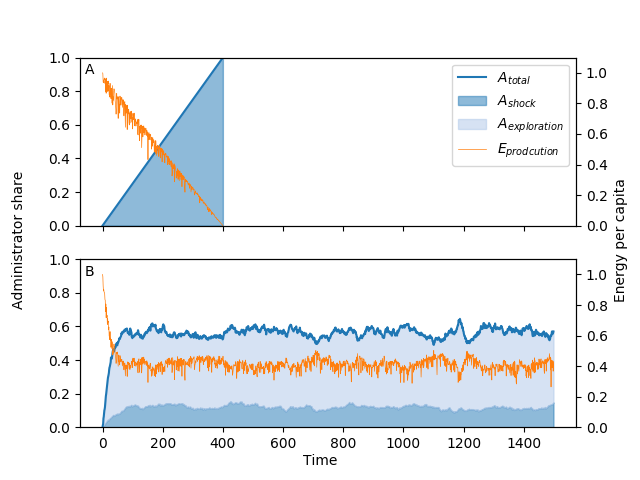
\includegraphics[width=\linewidth]{../figures/Admin_Ecap_twocases.png}
    \caption{Exemplary network simulation of a Tainter like model according to the model description in \ref{sec:modeldesc}. Both simulations were run for a maximum of 1500 time steps. Blue curves show the share of administration in the network (light blue: Administration as result of decreased resource availability, dark blue: Administration resulting from exploration). Orange curves show the average energy produced per node. A) shows the typical development of a network reacting to shocks by changing one node from C to A. As a result, initially the share of administration rises slowly, due to high marginal returns on investments (shown by the orange curve) until each further node changed to administration, negatively affects the energy produced by the network. B) shows the development of a network with the interaction of tainter dynamic and exploration dynamic. After a short period of rapid increase in administration, the network reaches a stable fixpoint upon which the share of administration and energy production remain stable and fluctuates only as a result of random beta distributed reductions of energy access.}
    \label{fig:baseNetworkDev}
\end{figure}


\paragraph{Interplay between network characteristics. Conditions for a beneficial administration}

Find out realistic ranges of efficiency and link density in simplistic societies, in order to be able to discuss the graphic




\begin{figure}[htb]
    \centering
    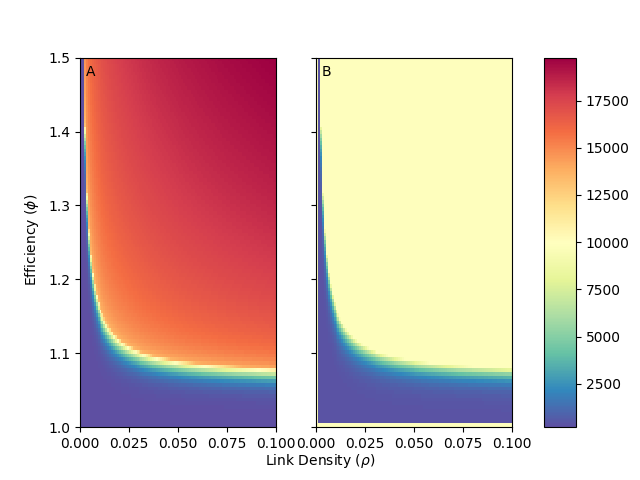
\includegraphics[width = \linewidth]{../figures/parscan_base0.png}
    \caption{Survival of a network with N = 400 as a function of exploration, link density and efficiency.}
    \label{fig:survival}
\end{figure}



\paragraph{Macroscopic approximation of original Tainter Dynamics}

\begin{figure}[htb]
    \centering
    \includegraphics[width = \linewidth]{../figures/comp_integration-model_exploration0.png}
    \caption{Survival of a network with N = 400 as a function of exploration, link density and efficiency.}
    \label{fig:survival}
\end{figure}

% P_e = 0 in order to leave out exploration term

\subsection{modified Tainter dynamics. Exploration}

\paragraph{model run description}

\paragraph{Low exploration results in highly increased survival times}

\paragraph{extension of macroscopic approximation}
